\subsection{Kommandozeilenprogramm Adobe-Illustrator-Designkonvertierung}
\label{Kommandozeilenprogramm Adobe-Illustrator-Designkonvertierung}
Wie bereits im Kapitel \ref{Der FreeDesign-Editor} \emph{Der FreeDesign-Editor} beschrieben, können die Kunden aus einer Vielzahl Designvorlagen eine Vorlage zur weiteren Gestaltung wählen. 
Diese Vorlagen werden von der hausinternen Grafikabteilung mit dem Programm \emph{Adobe Illustrator}, was eine Software zur Erstellung von Vektor-Grafiken ist \autocite[vgl.][]{Adobe:Illustrator}, erstellt und im SVG-Dateiformat gespeichert. Anschließend werden die SVG-Dateien durch einen Import-Prozess in das Easyprint-Shop-System importiert. Das FreeDesign-Projekt unterstützt diesen Prozess durch die Bereitstellung eines Kommandozeilenprogramms zur automatischen Konvertierung der SVG-Dateien, in ein Dateiformat welches durch den FreeDesign-Editor gelesen werden kann.  

Bereits im Architektur-Workshop wurde die direkte Integration des Quelltexts für die Kommandozeilenprogramme in den Quelltext des Editors bemängelt. 
Wie in \ref{fig:DesignImport} ist mitunter schwer zu trennen, welche Komponenten zum Kommandozeilenprogramm gehören und welche zum Editor. 
\begin{figure}[H]
    \centering
    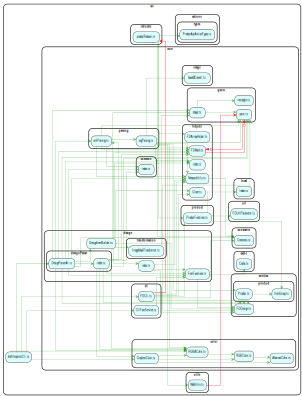
\includegraphics{diagrams/Ist-Architektur/draftImporter-analysis.pdf}
    \caption{Abhängigkeiten der Komponenten für das Kommandozeilenprogramm zur Konvertierung von Designs die mit Adobe-Illustrator erstellt wurden zu FreeDesign-Designs.}
    \label{fig:DesignImport}
\end{figure}


Durch die Umsetzung bestehen mehrere Programm.
\paragraph{Testbarkeit} 
Bei Änderung des Quelltextbasis müssen sowohl der FreeDesign-Editor als die Kommandozeilenprogramme getestet werden, auch wenn die Änderung nur ein Programm betrifft.
\paragraph{Gefahr von Quelltextleichen}
Unter Quelltextleichen ist Quelltext zu verstehen, der nicht ausgeführt wir \autocite[vgl.][292]{Martin2009}. Sollte das Importieren von Designvorlagen nicht mehr notwendig sein oder es wird ein alternativer Prozess gefunden, existiert weiterhin Quelltext im FreeDesign-Projekt, der das Projekt aufbläht und aufwändig entfernt werden sollte.
\newline
Folgende Bausteine wurden identifiziert, die für den DesignImport notwendig sind: 

\begin{multicols}{2}    
    \begin{enumerate}
    \item{API-Kommunikation}
    \item{Bildverarbeitung}
    \item{Cache}
    \item{Designstruktur}
    \item{Design-Parser}
    \item{Produktstruktur}
    \item{Farbstruktur}
    \item{JavaScript-Erweiterung}
    \item{Mathematik}
    \item{Maßeinheit-Konverter}
    \item{SVG-Parser}
    \item{Schriftverarbeitung}
    \item{XML-Parser}
\end{enumerate}
\end{multicols}